\documentclass{article}

\usepackage[utf8]{inputenc}
% \usepackage[utf8]{inputenc}
\usepackage{multicol}
\usepackage{dcolumn}
\usepackage[a4paper,top=3cm,bottom=3cm,left=1.5cm,right=1.5cm,marginparwidth=1.75cm]{geometry}
\usepackage{multicol}
\setlength{\columnsep}{0.5cm}
\usepackage{multirow}
\usepackage{amsmath}
\usepackage{graphicx}
\usepackage{hyperref}
\hypersetup{colorlinks=true,linkcolor=blue,filecolor=magenta,urlcolor=cyan,}
\usepackage{amsfonts}
\usepackage{mathtools}
\usepackage{lipsum}
\usepackage{float}
\usepackage{layout}
\usepackage{bm}

\usepackage{listings}
\usepackage{xcolor}
\definecolor{codegreen}{rgb}{0,0.6,0}
\definecolor{codegray}{rgb}{0.5,0.5,0.5}
\definecolor{codepurple}{rgb}{0.58,0,0.82}
\definecolor{backcolour}{rgb}{0.95,0.95,0.92}
\lstdefinestyle{mystyle}{
    backgroundcolor=\color{backcolour},
    commentstyle=\color{codegreen},
    keywordstyle=\color{blue},
    numberstyle=\tiny\color{codegray},
    stringstyle=\color{codepurple},
    basicstyle=\ttfamily\footnotesize,
    breakatwhitespace=false,
    breaklines=true,
    captionpos=b,
    keepspaces=true,
    numbers=left,
    numbersep=5pt,
    showspaces=false,
    showstringspaces=false,
    showtabs=false,
    tabsize=2
}
\lstset{style=mystyle}





\begin{document}










%TitlePage%TitlePage%TitlePage%TitlePage%TitlePage%TitlePage%TitlePage%TitlePage%TitlePage%TitlePage%TitlePage%TitlePage%TitlePage
\thispagestyle{empty}
\baselineskip25pt
\begin{center}
{\Large {\textbf{TitleTitleTitleTitleTitleTitleTitleTitleTitle \\Title}}}\\
\end{center}

\vfill
\baselineskip15pt
\begin{center}
{\em Computational Physics Term Project Report Submitted} \\
in Partial Fulfilment of the Requirements \\
for the course \
\vskip .30\baselineskip
{\large{\bf P52-Computational Physics}}
\end{center}
\baselineskip25pt

\vfill
\begin{center} {\bf {\em by}} \\
{\large{\bf ANANTHA PADMANABHAN M NAIR}} \\
Course Instructors:\\
\textbf{Dr. Subashis Basak\\
Dr. Prasanjit Samal}
\end{center}

\vfill
\begin{center}
\begin{figure}[h!]
\centering

\includegraphics[scale=0.2]{Images/logo1.jpg}
\end{figure}
 {\bf {\em to the }} \\
{\bf {\large School of Physical Sciences}} \\
{\bf {\large National Institute of Science Education and Research}} \\
{\bf Bhubaneswar} \\
{\bf \today} 
\end{center}
%TitlePage%TitlePage%TitlePage%TitlePage%TitlePage%TitlePage%TitlePage%TitlePage%TitlePage%TitlePage%TitlePage%TitlePage%TitlePage%










%Content Table Page%Content Table Page%Content Table Page%Content Table Page%Content Table Page%Content Table Page
\pagenumbering{roman}
\newpage
\newgeometry{top=2.5cm,bottom=2.5cm,left=3.5cm,right=3.5cm}
\begin{center}
 \tableofcontents  
 \newpage
 \listoffigures
 \listoftables 
\end{center}
\restoregeometry
%Content Table Page%Content Table Page%Content Table Page%Content Table Page%Content Table Page%Content Table Page



\newpage
\begin{center}
    \large{\textbf{TitleTitleTitleTitleTitleTitleTitle \\Title}}
\end{center}
\begin{abstract}
    We use Python to conduct a thorough investigation of the one-dimensional quantum harmonic oscillator (QHO) and its extensions in this computational physics research. We commence with the fundamental concepts of quantum physics and delve into the behavior of the QHO by calculating its eigenvalues and eigenvectors, offering a firm grasp of its inherent attributes. We then introduce other potentials, including the Hartree, Coulomb, and B88 potentials, and examine how they affect the energy spectrum and wavefunctions of the QHO system. By using numerical methods, such as the discrete Fourier transform (DFT), we examine how the system behaves in various potential landscapes and boundary conditions, providing new insights into its dynamics. Python has proven to be an effective and versatile tool for simulation and analysis during our examination, allowing for the flexible and efficient study of intricate quantum processes. This study advances our knowledge of quantum systems and their behavior in a variety of possible contexts by fusing theoretical ideas with computational techniques. It also provides insightful information for future research in quantum mechanics and computational physics.
\end{abstract}
\begin{multicols}{2}
\pagenumbering{arabic}






\section{\label{intro}Introduction}
One of the key pillars of quantum mechanics, the quantum harmonic oscillator (QHO) provides deep insights into the behavior of quantum systems and paves the way for many developments in theoretical physics and quantum computing. The QHO, which was first proposed in the early 20th century, became a key idea in the growth of quantum theory and completely changed our knowledge of particle motion and energy quantization.

The QHO model is based on the fundamentals of classical mechanics, in which a particle is subjected to a harmonic potential with a displacement from equilibrium that has a quadratic energy dependency. However, the Schrödinger equation, which defines the system's wavefunction evolution, governs the QHO's dynamics in quantum mechanics. We get a discrete spectrum of energy levels from the solutions to this equation, each of which is connected to a particular wavefunction or system eigenstate. These eigenstates provide a comprehensive description of the QHO's quantum mechanical behavior by forming an orthonormal basis spanning its Hilbert space.

We introduce the Python programming language as our main tool for numerical simulations and analysis, moving from theory to practice. Python's ease of use and readability enable academics from a variety of backgrounds to collaborate and share knowledge within the scientific community. We give a quick rundown of the main Python functionalities and study-relevant libraries, such as Matplotlib for data visualization, SciPy for scientific computing, and NumPy for numerical computations.
%%%%%%%%%%%%%%%%%%%%%%%%%%%%%%%%%%%%%%%%%%%%%%%%%%%%%%%%%%%%%%%%%%%%%%%%%%%%%%%%%%%%%%%%%%%%%%%%%%%%%%%%%%%%%%%%%%%%%%%%%%%%%%%%%%%%%%%%%%%%%%%%%%%%%%%%%%
\section{\label{theory}Theory and Background}

The main theory of this project revolves aroud the Schrodinger equation and its solution. The Schrodinger equation is given by:
\begin{equation}
    \hat{H}\psi = E\psi
\end{equation}

where $\hat{H}$ is the Hamiltonian operator, $\psi$ is the wavefunction and $E$ is the energy of the system. The differential form of the Schrodinger equation is given by:
\begin{equation}
    \hat{H}\psi = -\frac{\hbar^2}{2m}\nabla^2\psi + V(x,t)\psi = E\psi
\end{equation}

for our case we will restrict to the case where $V(x,t) = V(x)$ where the potentals depend only on the position of the particle. In uor study we will consider the case of a Quantum harmonic Oscillator. where the potential is given by:
\begin{equation}
    V(x) = \frac{1}{2}m\omega^2r^2
\end{equation}
where $\omega$ is the frequency of the oscillator, m is the mass of the particle and r is the distance from the equilibrium position. In our case we will consider the units where $\hbar = 1$ and $m = 1$. So the Hamiltonian operator for the QHO is given by:
\begin{equation}
    \hat{H} = -\frac{1}{2}\nabla^2 + \frac{1}{2}r^2
\end{equation}

From here we will add few additional potentials to the QHO and study the effect of these potentials on the energy spectrum and wavefunctions of the system. 
The problems that we are focusing on are:
\begin{itemize}
    \item Quantum Harmonic Oscillator
    \item Quantum Harmonic Oscillator half harmonic potential
    \item Quantum Harmonic Oscillator in soft Coulomb Potential
    \item One dimentional DFT Code
    \item 2-Dimentional Harmonic Oscillator
\end{itemize}


\subsection{\label{QHO}Quantum Harmonic Oscillator}
Here we will be solving the differential equation given by:
\begin{equation}
    -\frac{1}{2}\frac{d^2\psi}{dx^2} + \frac{1}{2}x^2\psi = E\psi
\end{equation}

The potental is defined in the range of $-\infty$ to $\infty$. The solution to this differential equation is given by the Hermite polynomials. which is already calculated.
Proper solutions exist for this  differential equation iff its Energy is one of the allowed values. The allowed values of the energy is calculated by the eigenvalue of the Hamiltonian operator where the H is represented as a matrix.

\subsection{\label{QHOHP}Quantum Harmonic Oscillator half harmonic potential}

Here only the positive values of x are considered. The potential is given by:
\begin{equation}
    V(x) = \frac{1}{2}x^2 \text{ for } x > 0
\end{equation}
and $\inf$ otherwise.
So the solutions in the negative part of the x axis is zero.




\subsection{\label{QHOSC}Quantum Harmonic Oscillator in soft Coulomb Potential}

Here the potential is given by:
\begin{equation}
    V(x) = \frac{1}{2}x^2 + \frac{1}{\sqrt{1+x^2}}
\end{equation}







\subsection{\label{DFT}One dimentional DFT Problem}

In the DFT, we will be considering the Hamiltonian operator given by:
\begin{equation}
    \hat{H} = -\frac{1}{2}\nabla^2 + \frac{x^2}{2}  + V_{Ha}(x) + V_{X}^{LDA} (x)
\end{equation}

In this case will o include both the Coulomb or Hartree interaction as well as LDA exchange, both of which are density functionals. So, we need to calculate the electron density and the exchange potential. For that we need the wavefunctions $\Psi (x)$ to be normalized. The normalization condition is given by:
\begin{equation}
    \int_{-\infty}^{\infty} |\Psi(x)|^2 dx = 1
\end{equation}

Now the electron density is given by:
\begin{equation}
    n(x) = \sum_{n=1} f_n |\Psi_n(x)|^2
\end{equation}

Where $f_n$ is the occupation number. The lowest energy levels will be occupied by the electrons. Up to two electrons—one with spin up and one with spin down—fit into each state. Thus, a state can have zero, one, or two electrons.

\subsubsection{\label{Hartree}Exchange Energy}

An approximation of the influence of electron interactions on the electronic energy is the exchange-correlation functional. We disregard association in order to keep things simple because it is more laborious to describe than fascinating to do so. The exchange functional in the local density approximation (LDA), then, is as follows:

\begin{equation}
    E_{X}^{LDA} (x) = -\frac{3}{4}(\frac{3}{\pi})^{(1/3)} \int n(x')^{4/3} dx'
\end{equation}

The derivative of the energy with respect to the density is the definition of the potential corresponding to each energy phrase in the Kohn-Sham equations. Consequently, the derivative of the exchange energy with respect to density yields the exchange potential:

\begin{equation}
    V_{X}^{LDA} (x) = -\frac{dE_{X}^{LDA} (x)}{dn(x)} = -(\frac{3n(x)}{\pi})^{(1/3)}
\end{equation}



\subsubsection{\label{Coulomb}Hartree Energy}

Doing the same procedure we can write the hartree potential as:

\begin{equation}
    V_{Ha} (x) = \int \frac{n(x')}{\sqrt{|x-x'|^2+1}} dx'
\end{equation}



\subsection{\label{2DQHO}2-Dimentional Harmonic Oscillator}

The Equation thet we want solve is:
\begin{equation}
    -\frac{1}{2}\nabla^2\psi + \frac{1}{2}(x^2 + y^2)\psi = E\psi
\end{equation}


We can split the Energy into two parts $E = E_x + E_y$ where $E_x$ and $E_y$ are the energies in the x and y directions respectively. The solution to this differential equation is given by the product of the individual solutions to the x and y wavefunctions.

\subsubsection{Seperation of Variables}

Expanding the laplacian operator in the above equation we get::
\begin{equation}
    -\frac{1}{2}(\frac{\partial^2\psi}{\partial x^2} + \frac{\partial^2\psi}{\partial y^2}) + \frac{1}{2}(x^2 + y^2)\psi = (E_x + E_y)\psi
\end{equation}



We ca clearly see that the solution of the above equation is the product of the individual solutions to the x and y wavefunctions. So we can write the wavefunction as:
\begin{equation}
    \psi(x,y) = X(x)Y(y)
\end{equation}

on substituting it into the schrodinger equation, we get the splitted equation as:

\begin{eqnarray}
    \frac{1}{X}\frac{\partial^2 X}{\partial x^2} - (x^2 + 2E_x) = k\\
    \frac{1}{Y}\frac{\partial^2 Y}{\partial y^2} - (y^2 + 2E_y) = -k
\end{eqnarray}

So on solving these two equations seperately, we will get the wavefunction of the 2-Dimentional Harmonic Oscillator.

%%%%%%%%%%%%%%%%%%%%%%%%%%%%%%%%%%%%%%%%%%%%%%%%%%%%%%%%%%%%%%%%%%%%%%%%%%%%%
%%%%%%%%%%%%%%%%%%%%%%%%%%%%%%%%%%%%%%%%%%%%%%%%%%%%%%%%%%%%%%%%%%%%%%%%%%%%%
\section{\label{expsetup}Numerical Proedures and Computational Setup}

\subsection{\label{Python}Python and its Libraries}
For this project we will be using Python as our main tool for numerical simulations and analysis. We will mostly be using the following libraries:
\begin{itemize}
    \item NumPy: NumPy is a library for the Python programming language that adds support for large, multi-dimensional arrays and matrices, along with a large collection of high-level mathematical functions to operate on these arrays.
    \item SciPy: SciPy is a free and open-source Python library used for scientific and technical computing. It is a collection of mathematical algorithms and convenience functions built on the NumPy extension of Python.
    \item Matplotlib: Matplotlib is a plotting library for the Python programming language and its numerical mathematics extension NumPy. It provides an object-oriented API for embedding plots into applications using general-purpose GUI toolkits like Tkinter, wxPython, Qt, or GTK.
\end{itemize}


\subsection{For the Solution of the QHO with simple potentials}

For the solution of the QHO with soft Coulomb potential and half harmonic potential, we will be using the following procedure:
\begin{itemize}
    \item We will first calculate the Hamiltonian matrix for the given potential.
    \item We will then calculate the eigenvalues and eigenvectors of the Hamiltonian matrix.
    \item The eigenvalues will give us the energy levels of the system and the eigenvectors will give us the wavefunctions of the system.
    \item We will then plot the energy levels and the wavefunctions of the system.
\end{itemize}


The second derivative matrix is obtained using the finite element method and the potential matrix is the matrix with only the potential values in the diagonal. The Hamiltonian matrix is then obtained by adding the kinetic energy matrix and the potential matrix. A demonstration of the Hamiltonian matrix is shown below:

\begin{lstlisting}[language=Python]
    import numpy as np
    '''
    Grid points
    '''
    n=600
    x = np.linspace(-5,5,n)
    h = x[1]-x[0] 
    
    
    '''
    Second derivative matrix
    '''
    D=(-np.eye(n)+np.diagflat(np.ones(n-1),1))/h
    D2=D.dot(-D.T)
    D2[-1,-1]=D2[0,0]
    
    
    '''
    Potential energy matrix
    '''
    def V_half(x):    # half harmonic oscillator potential
        if x<0:
            return 10000000000
        else:
            return 0.5*x**2
    
    V_half = np.array([V_half(xi) for xi in x])
    V_half = np.diagflat(V_half)
    # print(V_half)
    '''
    Find the eigenvalues and eigenvectors
    '''
    Energy_half,psi_half = np.linalg.eigh(-D2/2 + V_half)
\end{lstlisting}





The Eigen values and Eigen vectors are obtained using the  function \texttt{np.linalg.eigh} in the numpy library.



\subsection{For the One dimentional DFT Problem}

For the One dimentional DFT problem we will be implementing the Kaun-Sham equations. A similar approach for the calculation of the hamiltonian is taken as in the previous case. The electron density is calculated using the wavefunctions and the exchange potential is calculated using the electron density. The exchange potential is then used to calculate the exchange energy. The Hartree potential is calculated using the electron density and the Hartree energy is calculated using the Hartree potential. The total energy is then calculated using the exchange energy and the Hartree energy. Here we have used a sef consistancy loop for the calculation of the solution of the wavefunctions. The self consistancy code is given below: (Here the hartree potentials and the exchange potentials are calculated. only the self consistancy loop is shown here)

\begin{lstlisting}{language = Python}
    nx = np.zeros(n)

    tolerence = 1e-6
    
    # Running the loop once to get the initial values of the energies
    hartree_energies_0 = get_hatree(nx,x)
    exchange_energies_0 = get_exchange_energy(nx,x)
    H=-D2/2+np.diagflat(exchange_energies_0[1]+hartree_energies_0[1]+x*x)
    energy_0, psi_0= np.linalg.eigh(H)
    nx_0=get_nx(num_electron,psi_0,x)
    steps = 1
    
    while True:
        hartree_energies_1 = get_hatree(nx_0,x)
        exchange_energies_1 = get_exchange_energy(nx_0,x)
        H=-D2/2+np.diagflat(exchange_energies_1[1]+hartree_energies_1[1]+x*x)
        energy_1, psi_1= np.linalg.eigh(H)
        nx_1=get_nx(num_electron,psi_1,x)
        if abs(energy_1[0] - energy_0[0]) < tolerence:
            print(f"converged after {steps} steps" )
            break
        elif steps > 1000:
            print(f"Did not converge after {steps} steps. Exiting.")
            break
        else:
            energy_0 = energy_1
            psi_0 = psi_1
            nx_0 = nx_1
            steps += 1

\end{lstlisting}    
    


\subsection{For the 2-Dimentional Harmonic Oscillator}

For solving the 2-D harmonic oscillator, we are using the RK4 method to solve the differential equation. The RK4 is implemented seperately for the x and y directions. for the RK4, the second order equation is split into two first order coupled equations by substituting dX/dx = f for eg. The RK4 method is then used to solve the two first order equations. Then the resulting products for the x and y directions are multiplied to get the wavefunction of the 2-D harmonic oscillator. As we are using the units where $\hbar = 1$ and $m = 1$, we know, the energy levels are given by $E = E_x + E_y$ where $E_x$ and $E_y$  are odd multiples of $\frac{1}{2}$. So, this energy levels that we will be using.


\subsection{The RK4 Method}

The genralised form of the RK4 method is used for solving a set of coupled differential equationsof the form:
\begin{equation}
    \frac{d\vec{y}}{dx} = \vec{f}(x,y)
\end{equation}
 
where $\frac{d\vec{y}}{dx}$ represents the set of equations $\{ y_1(y_1,y_2,y3,...x) ,y_2(y_1,y_2,y3,...x) , \},y_1(y_3,y_2,y3,...x),...$  and the $\vec{f}(x,y)$ represents the set of equations $\{ f_1(\vec{y},x),f_2(\vec{y},x),f_3(\vec{y},x),... \}$. Here the Rk4 equations are:
\begin{eqnarray}
    k_1 = h\vec{f}(x_n,y_n)\\
    k_2 = h\vec{f}(x_n + \frac{h}{2},y_n + \frac{k_1}{2})\\
    k_3 = h\vec{f}(x_n + \frac{h}{2},y_n + \frac{k_2}{2})\\
    k_4 = h\vec{f}(x_n + h,y_n + k_3)\\
    y_{n+1} = y_n + \frac{k_1 + 2k_2 + 2k_3 + k_4}{6}
\end{eqnarray}

This is done in a loop for the required number of steps ans convergence. 
%%%%%%%%%%%%%%%%%%%%%%%%%%%%%%%%%%%%%%%%%%%%%%%%%%%%%%%%%%%%%%%%%%%%%%%%%%%%%
%%%%%%%%%%%%%%%%%%%%%%%%%%%%%%%%%%%%%%%%%%%%%%%%%%%%%%%%%%%%%%%%%%%%%%%%%%%%%
\section{\label{observations}Solutions to the Quantum Harmonic Oscillator Problem}


The obtained results of the solution of QHO schrodinger equation are shown below. The energy levels and the wavefunctions are plotted for the QHO, QHO with half harmonic potential and QHO with soft Coulomb potential and the rest are shown in the coming sections.


\subsection{\label{QHO_1}Particle in Harmonic Potential}

The Plot of the usual harmonic oscillator is shown in the figure-\ref{usualqho}


\begin{figure}[H]
    \centering
    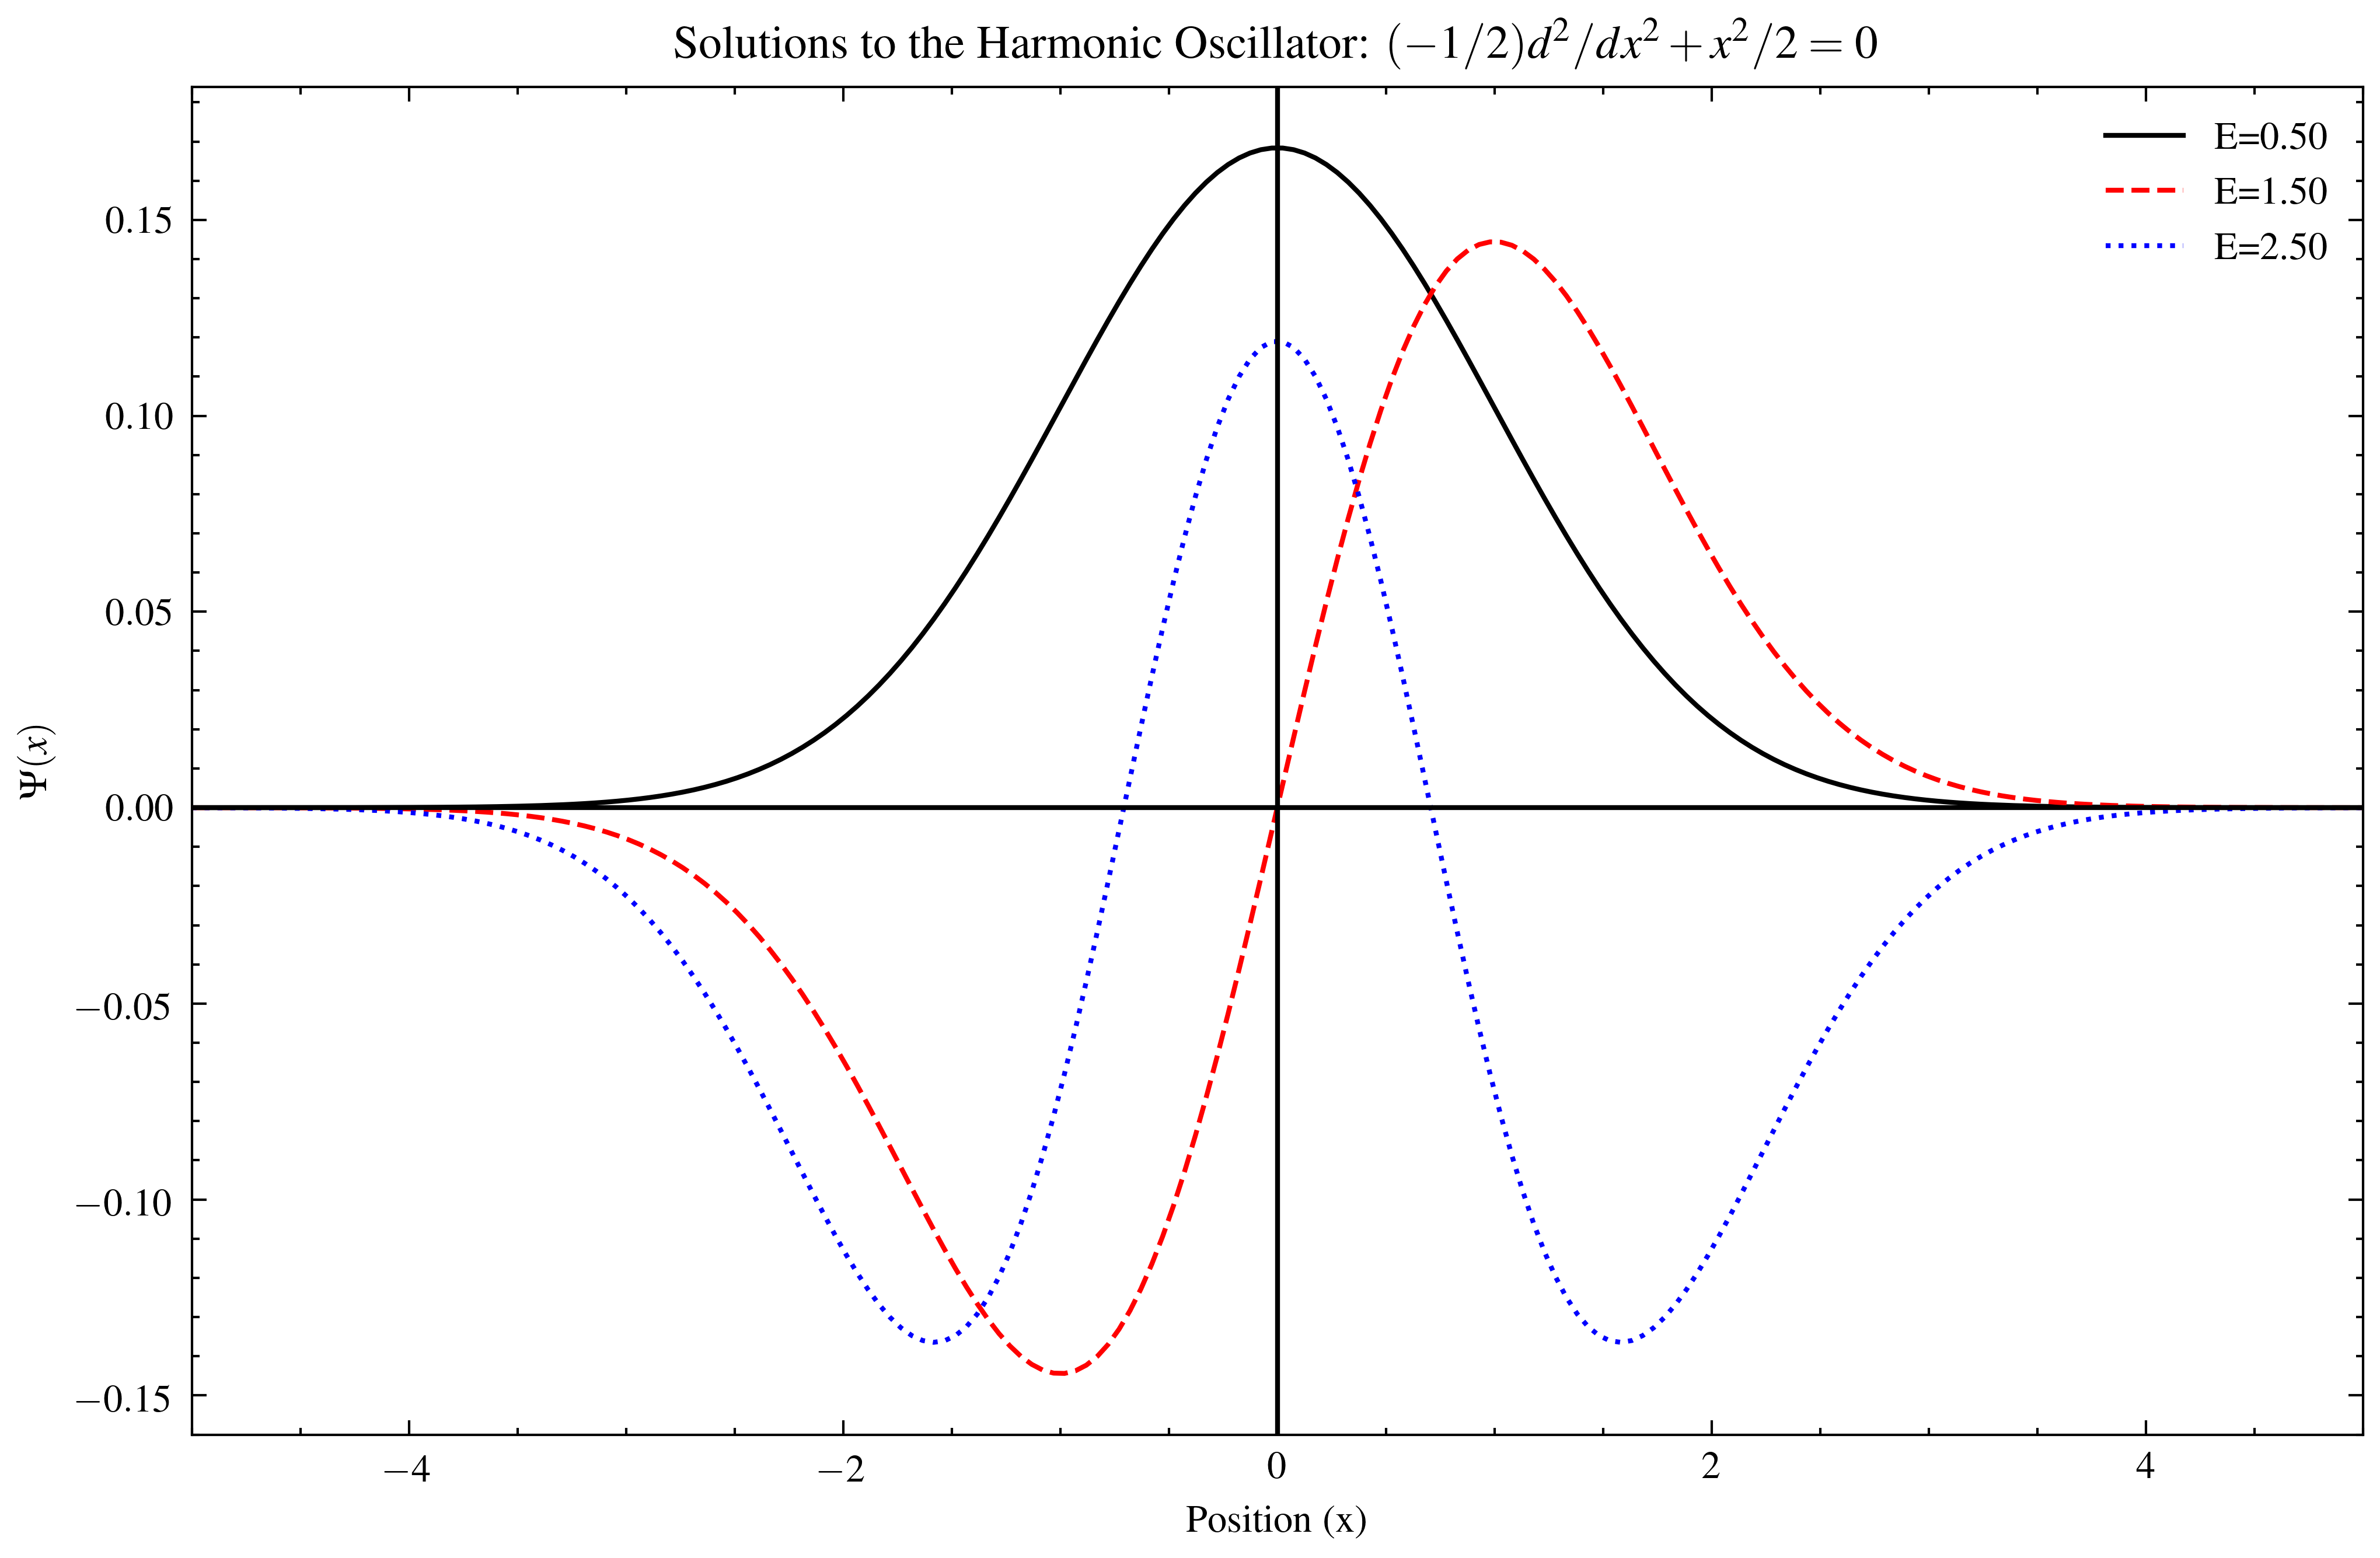
\includegraphics[width = \columnwidth]{Images/usual_QHO.png}
    \caption{Energy levels and wavefunctions of the Quantum Harmonic Oscillator for n = 0 to 2-\cite{python}}
    \label{usualqho}
\end{figure}

Here we can see the eigrnvalues of energy and the eigenvectors. This problem is analytically solved and we know that their solutions are hermite polynomials. In the figure, only the first 3 states are shown. These values of the energies that is $E_0 = 0.5$, $E_1 = 1.5$ and $E_2 = 2.5$, we will be using in the 2D-QHO Problem.




\subsection{Particle in Half Harmonic Potential}

The Plot of the QHO with half harmonic potential is shown in the figure-\ref{halfqho}

\begin{figure}[H]
    \centering
    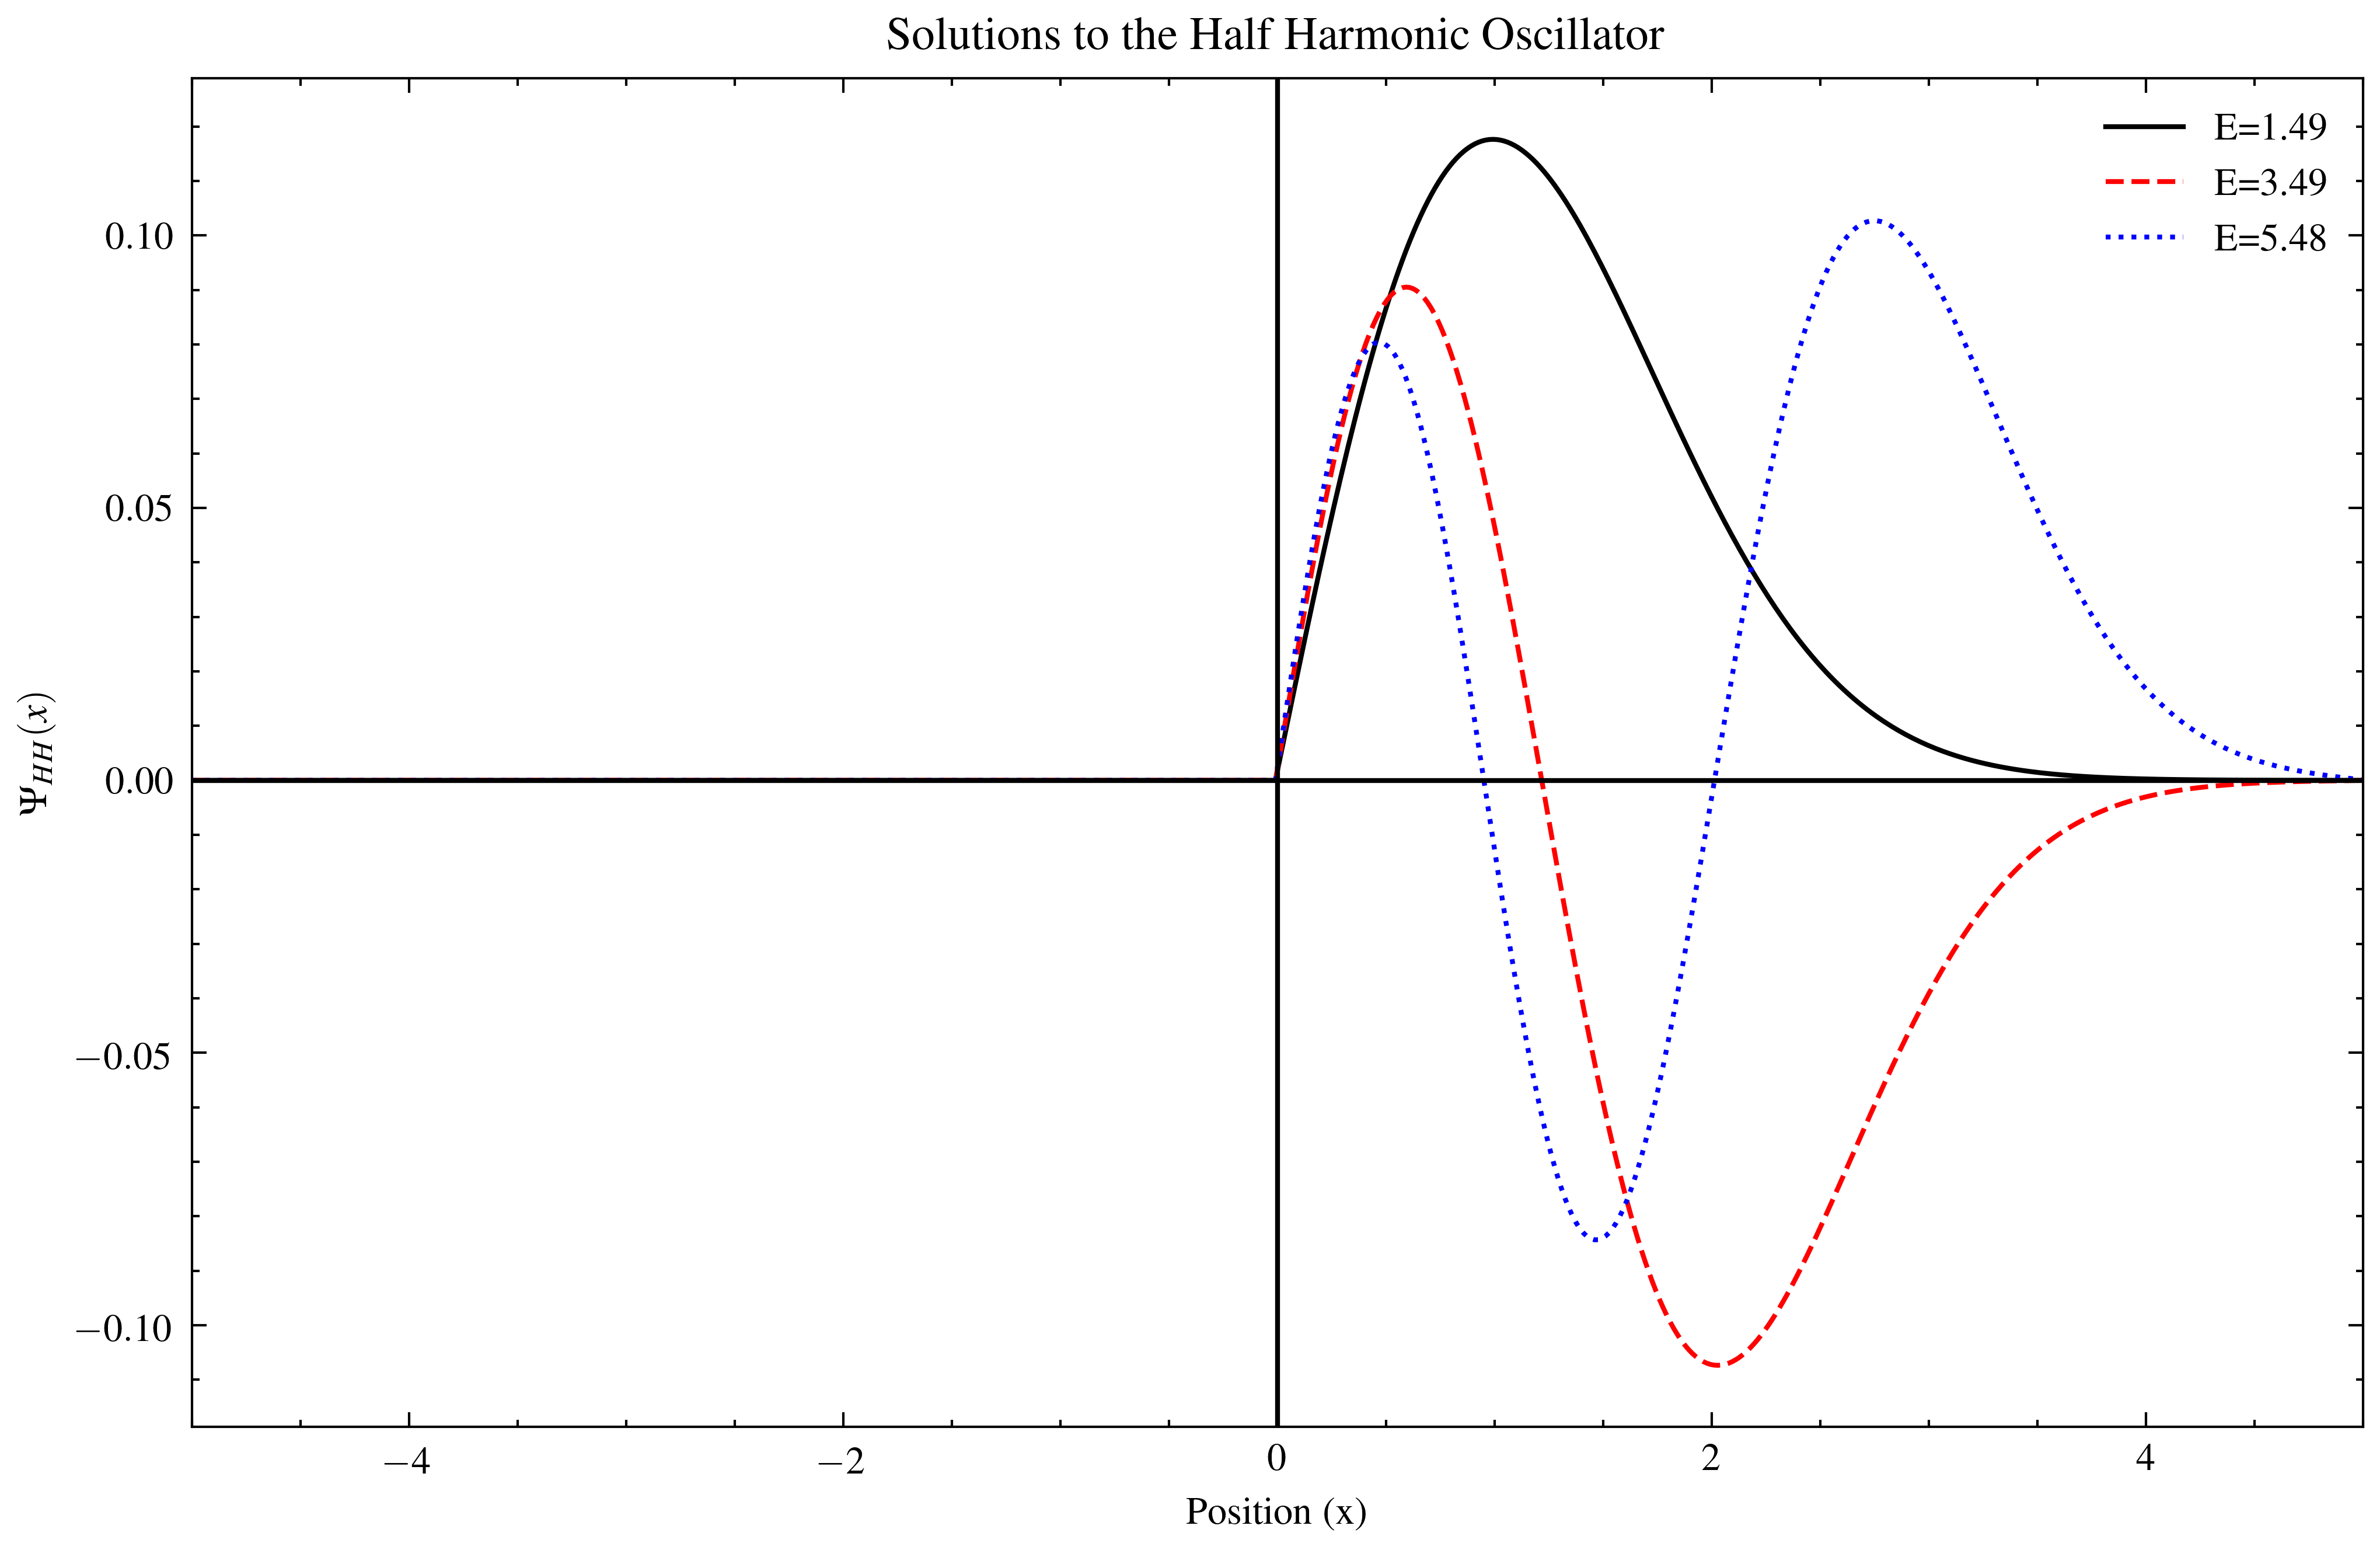
\includegraphics[width = \columnwidth]{Images/half_harmonic.png}
    \caption{Solutions to the half harmonic potential problem in QM}
    \label{halfqho}
\end{figure}

Here we can se that only the solutions of the usual QHO which has the wave function value 0 at the point x=0 are allowed.


\subsection{Particle in Soft Coulomb Potential}


The Plot of the QHO in soft Coulomb potential is shown in the figure-\ref{coulombqho}

\begin{figure}[H]
    \centering
    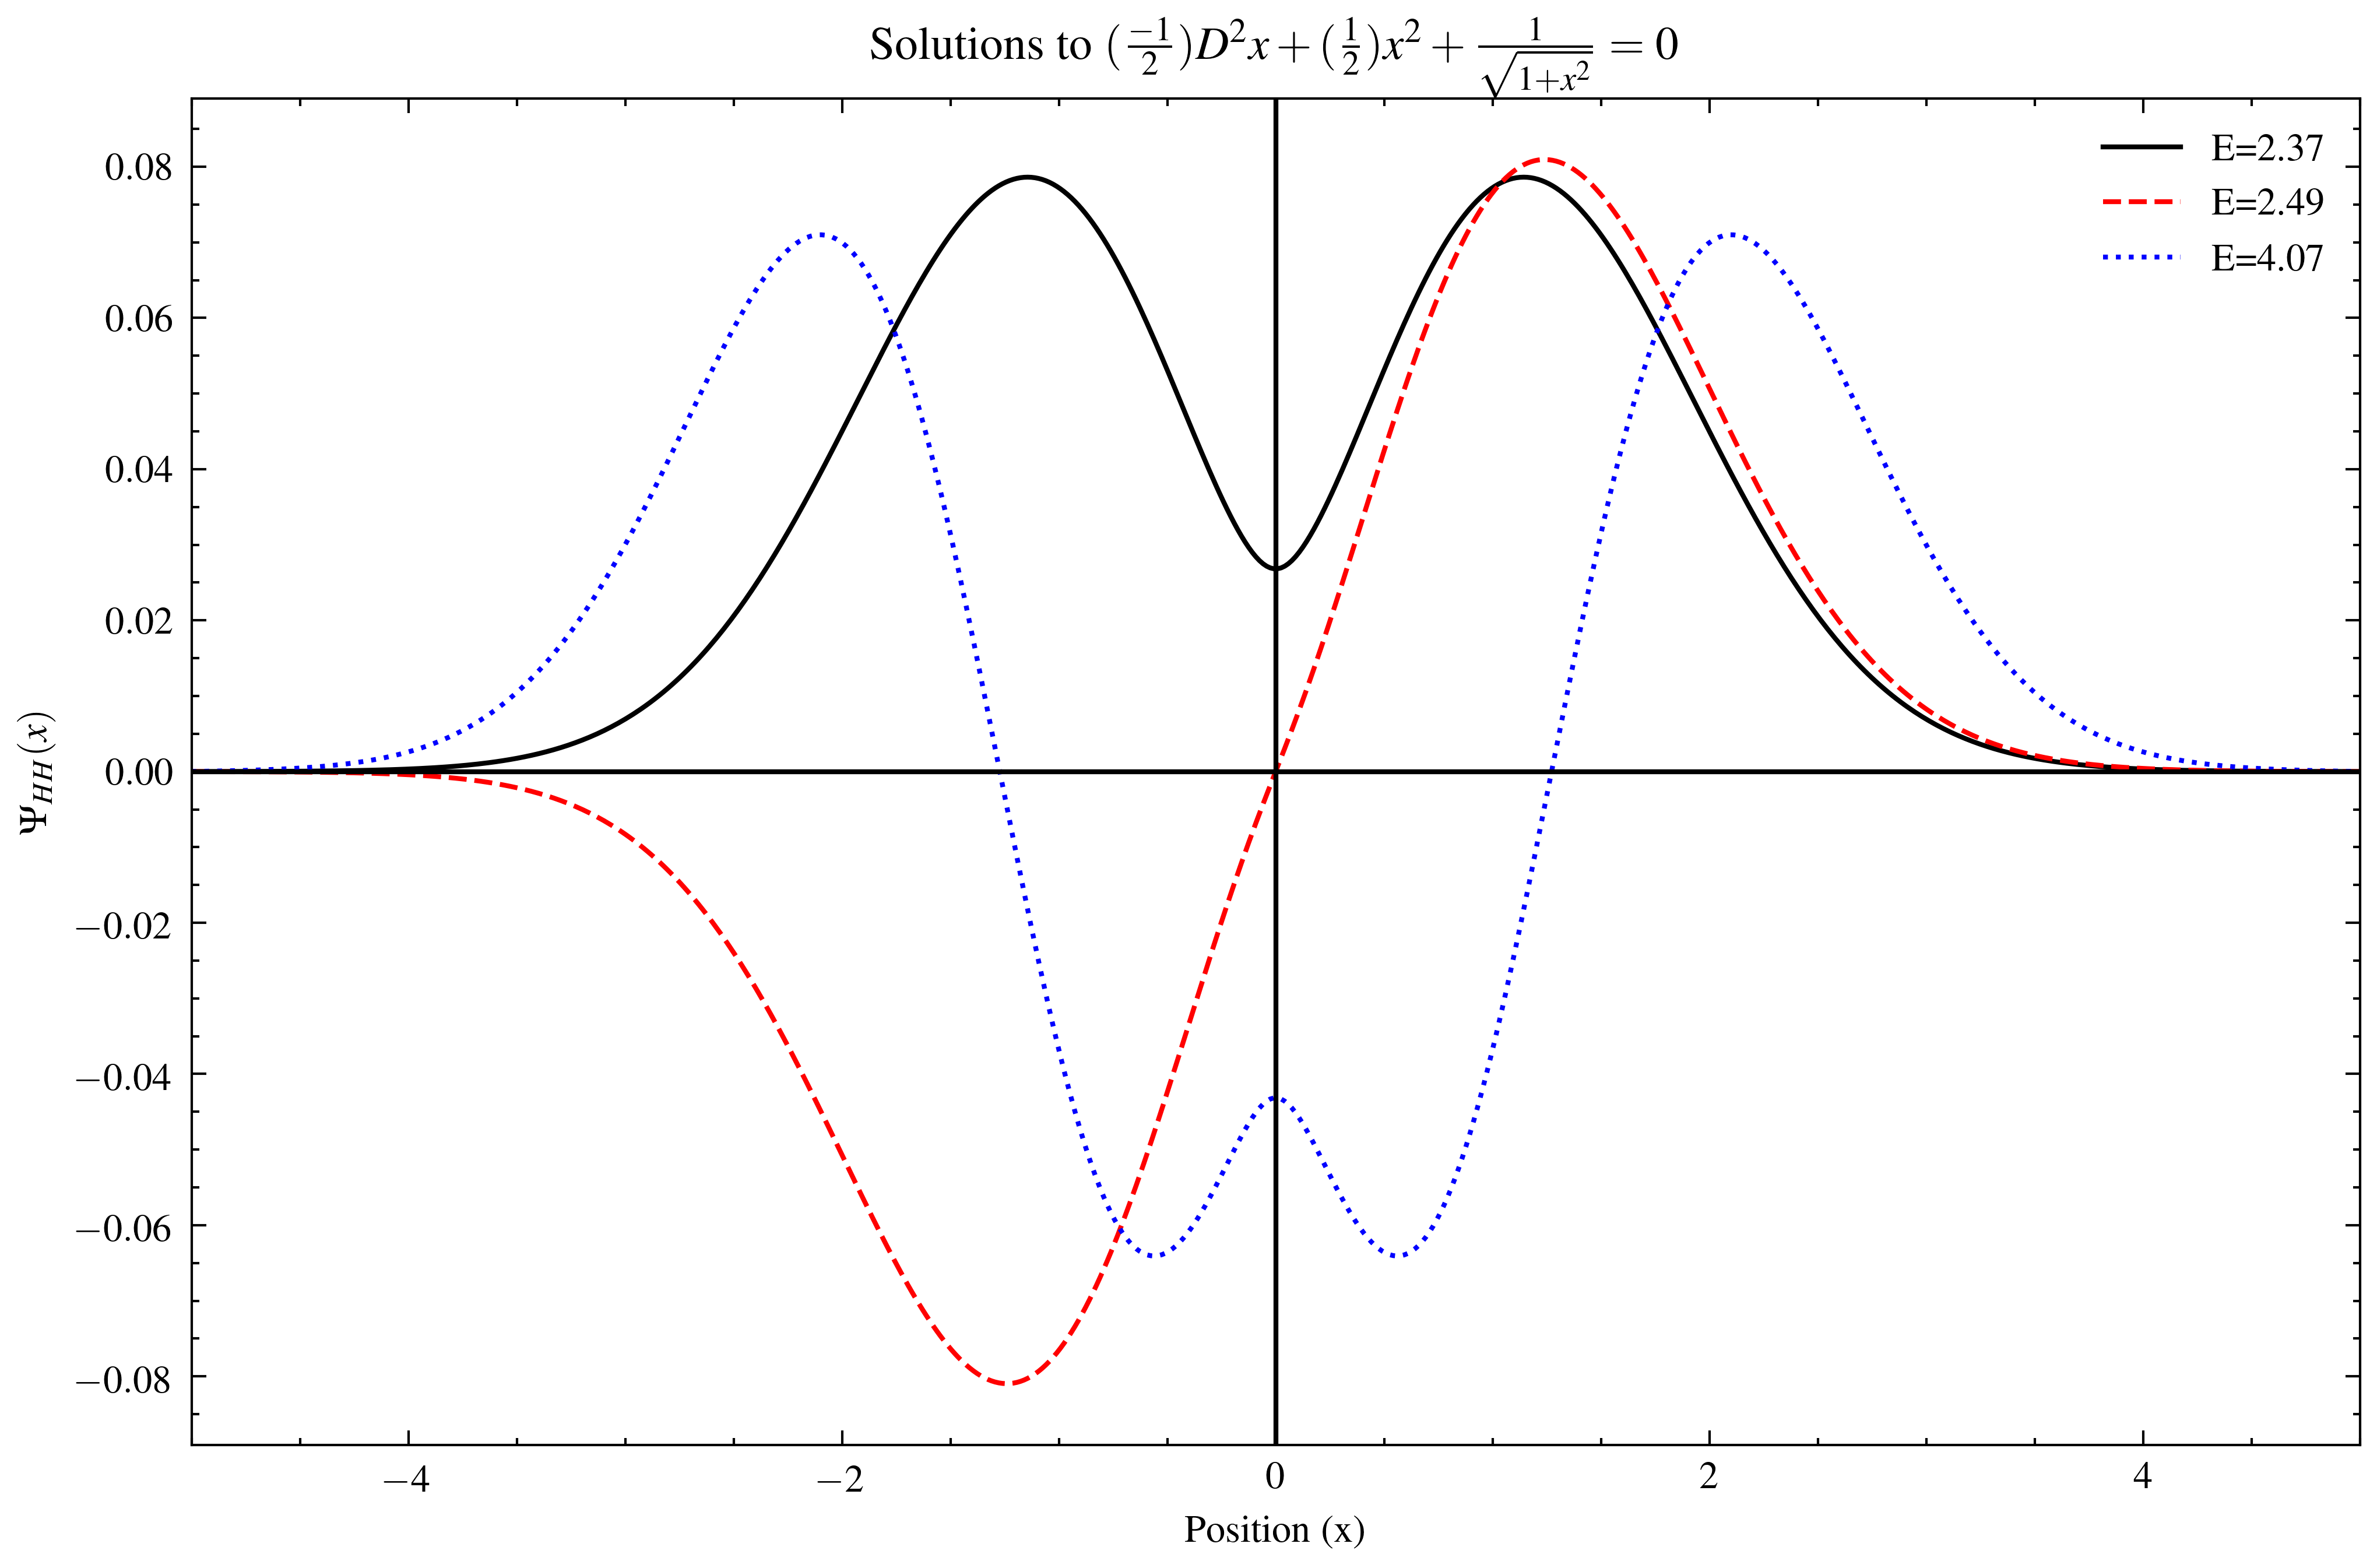
\includegraphics[width = \columnwidth]{Images/soft_coulomb.png}
    \caption{Solutions to the QHO in soft Coulomb potential}
    \label{coulombqho}
\end{figure}

Here we can see that the change in the Energy of the states and the wavefunctions of the system. The energy levels are shifted and the wavefunctions are also changed.The wavefunctions are more spread out in the case of the soft Coulomb potential. This is due to the fact that the potential is more spread out in the case of the soft Coulomb potential.


\subsection{One dimentional DFT Problem with LDA potential and Hartree Energy}



The plot of the number density for 17 electrons in the 1D DFT problem is shown in the figure-\ref{numden}

\begin{figure}[H]
    \centering
    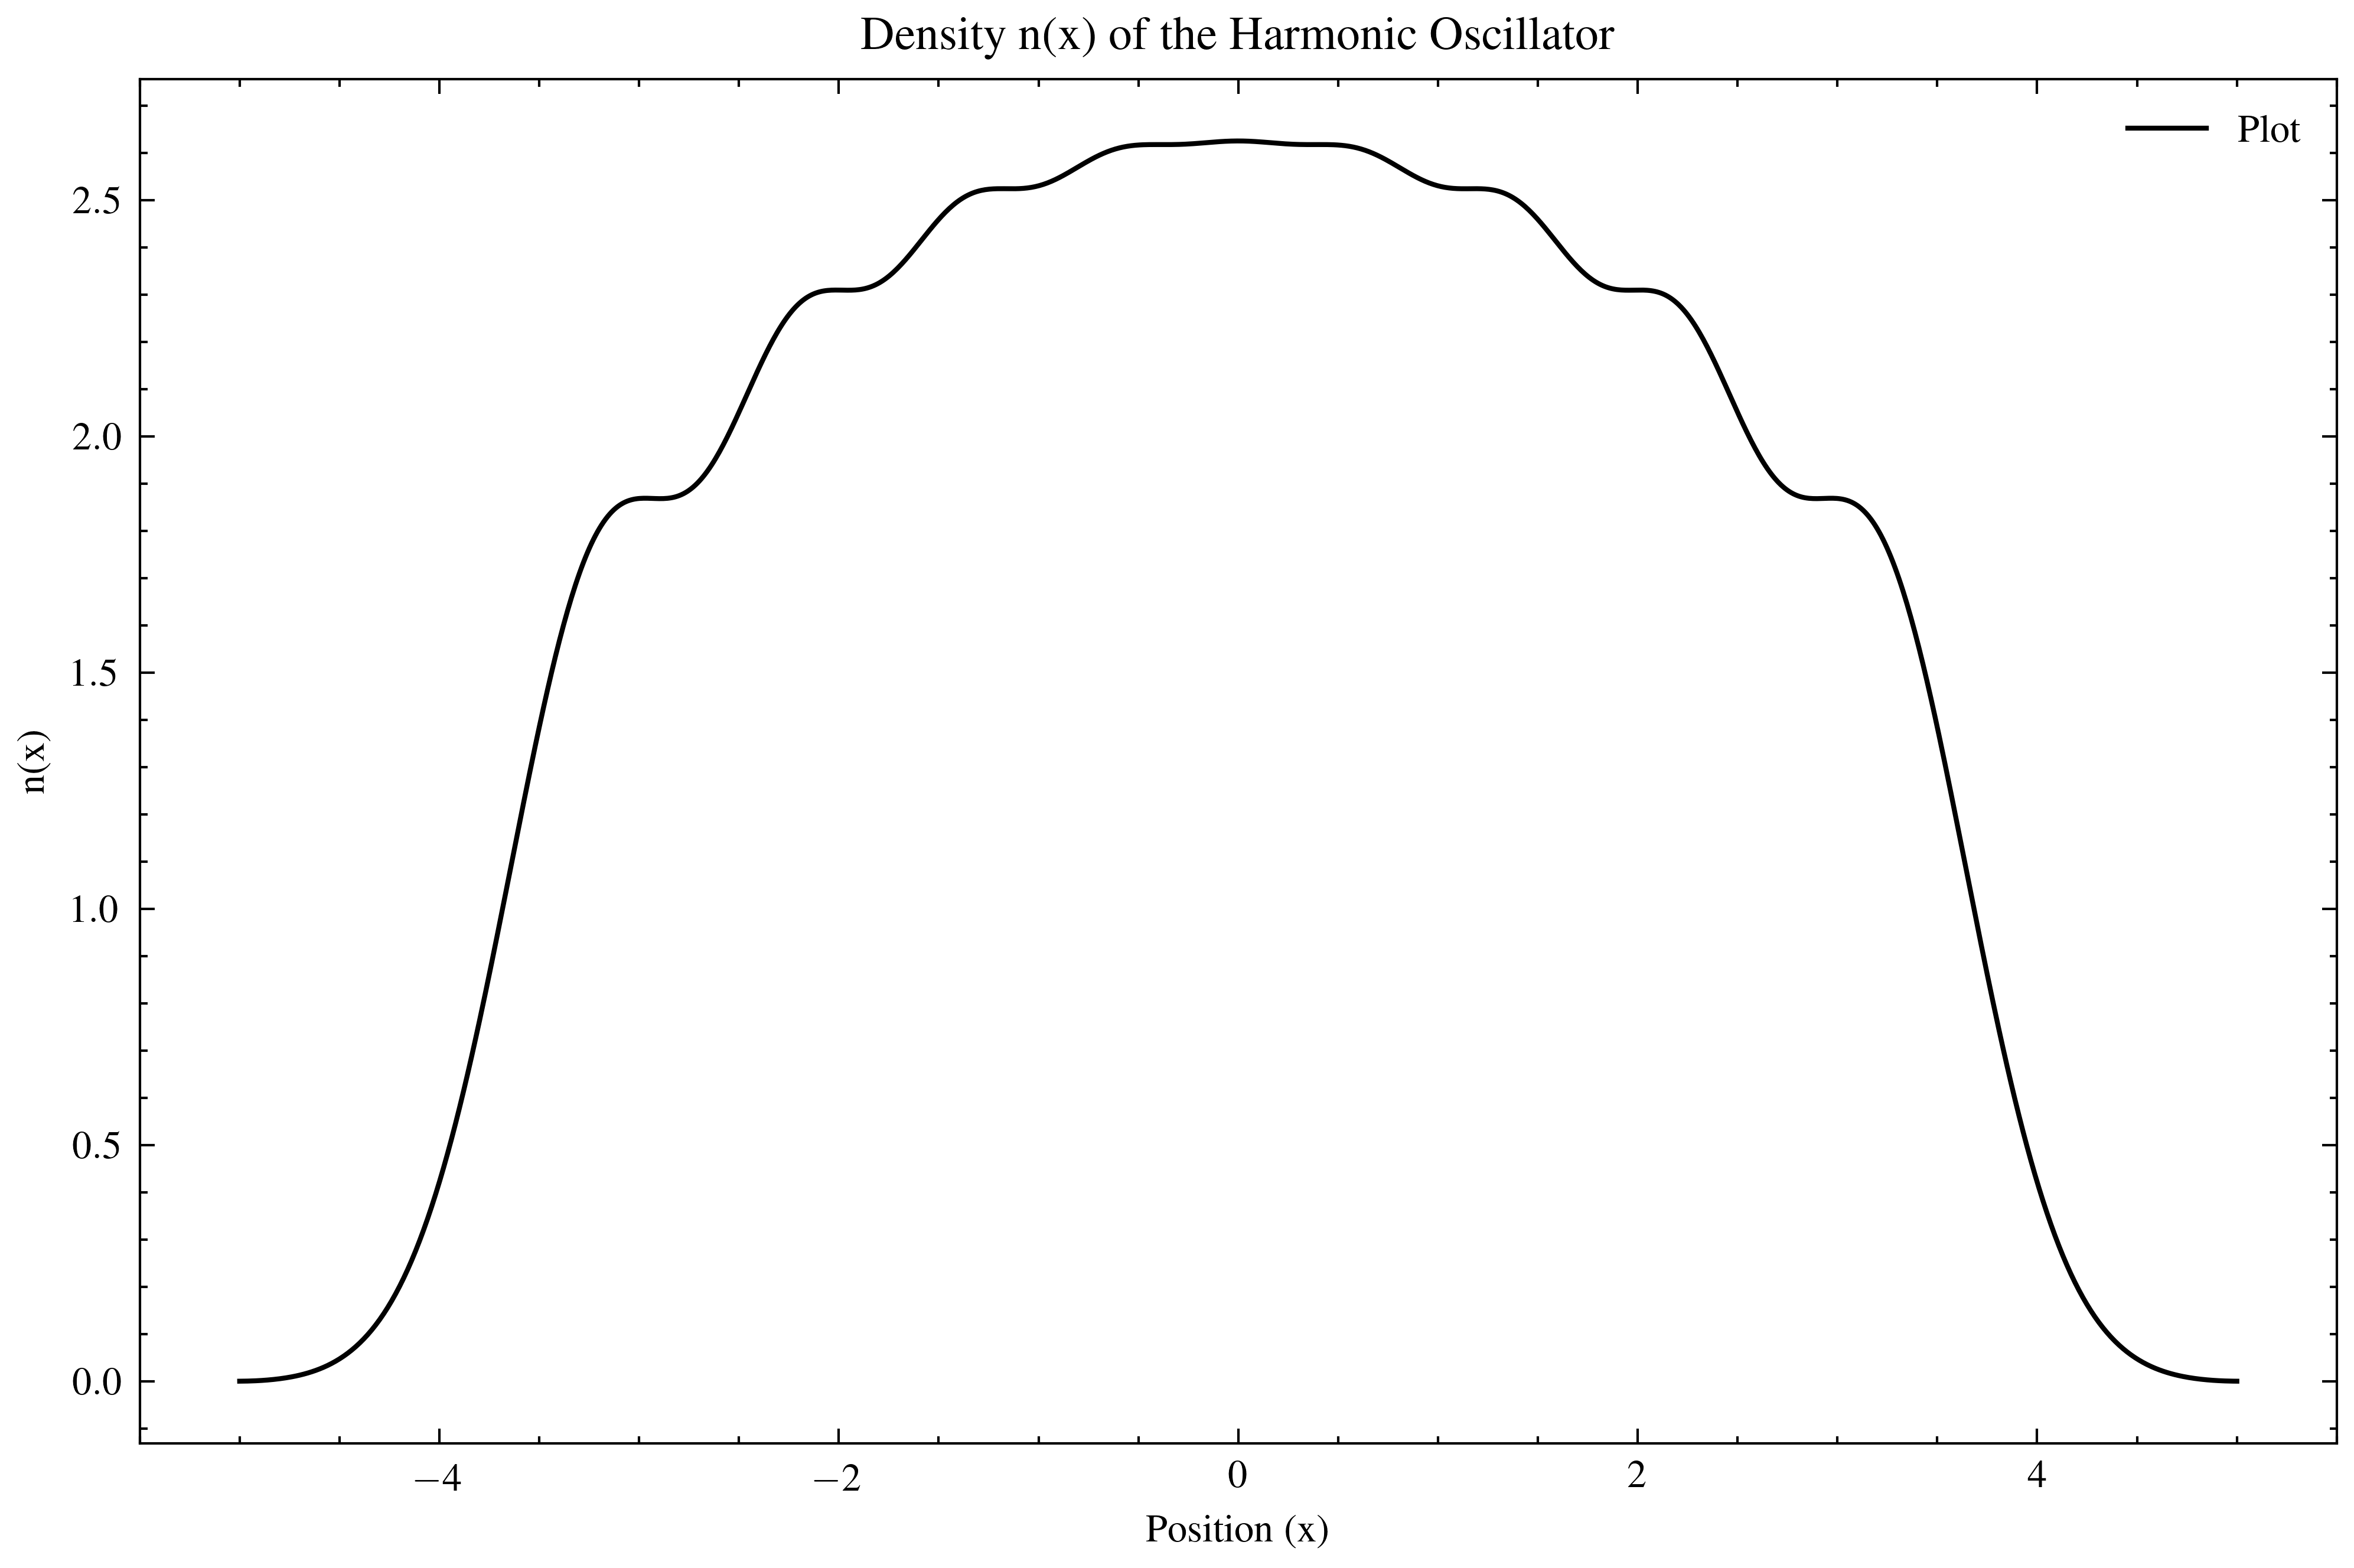
\includegraphics[width = \columnwidth]{Images/density.png}
    \caption{Number density n(x) of the electrons in the 1D DFT problem. The number of electrons used here is 17}
    \label{numden}
\end{figure}

The plot of the Solutions to the 1D DFT problem with LDA potental and Exchange Energy is shown in the figure-\ref{1d_dft}

\begin{figure}[H]
    \centering
    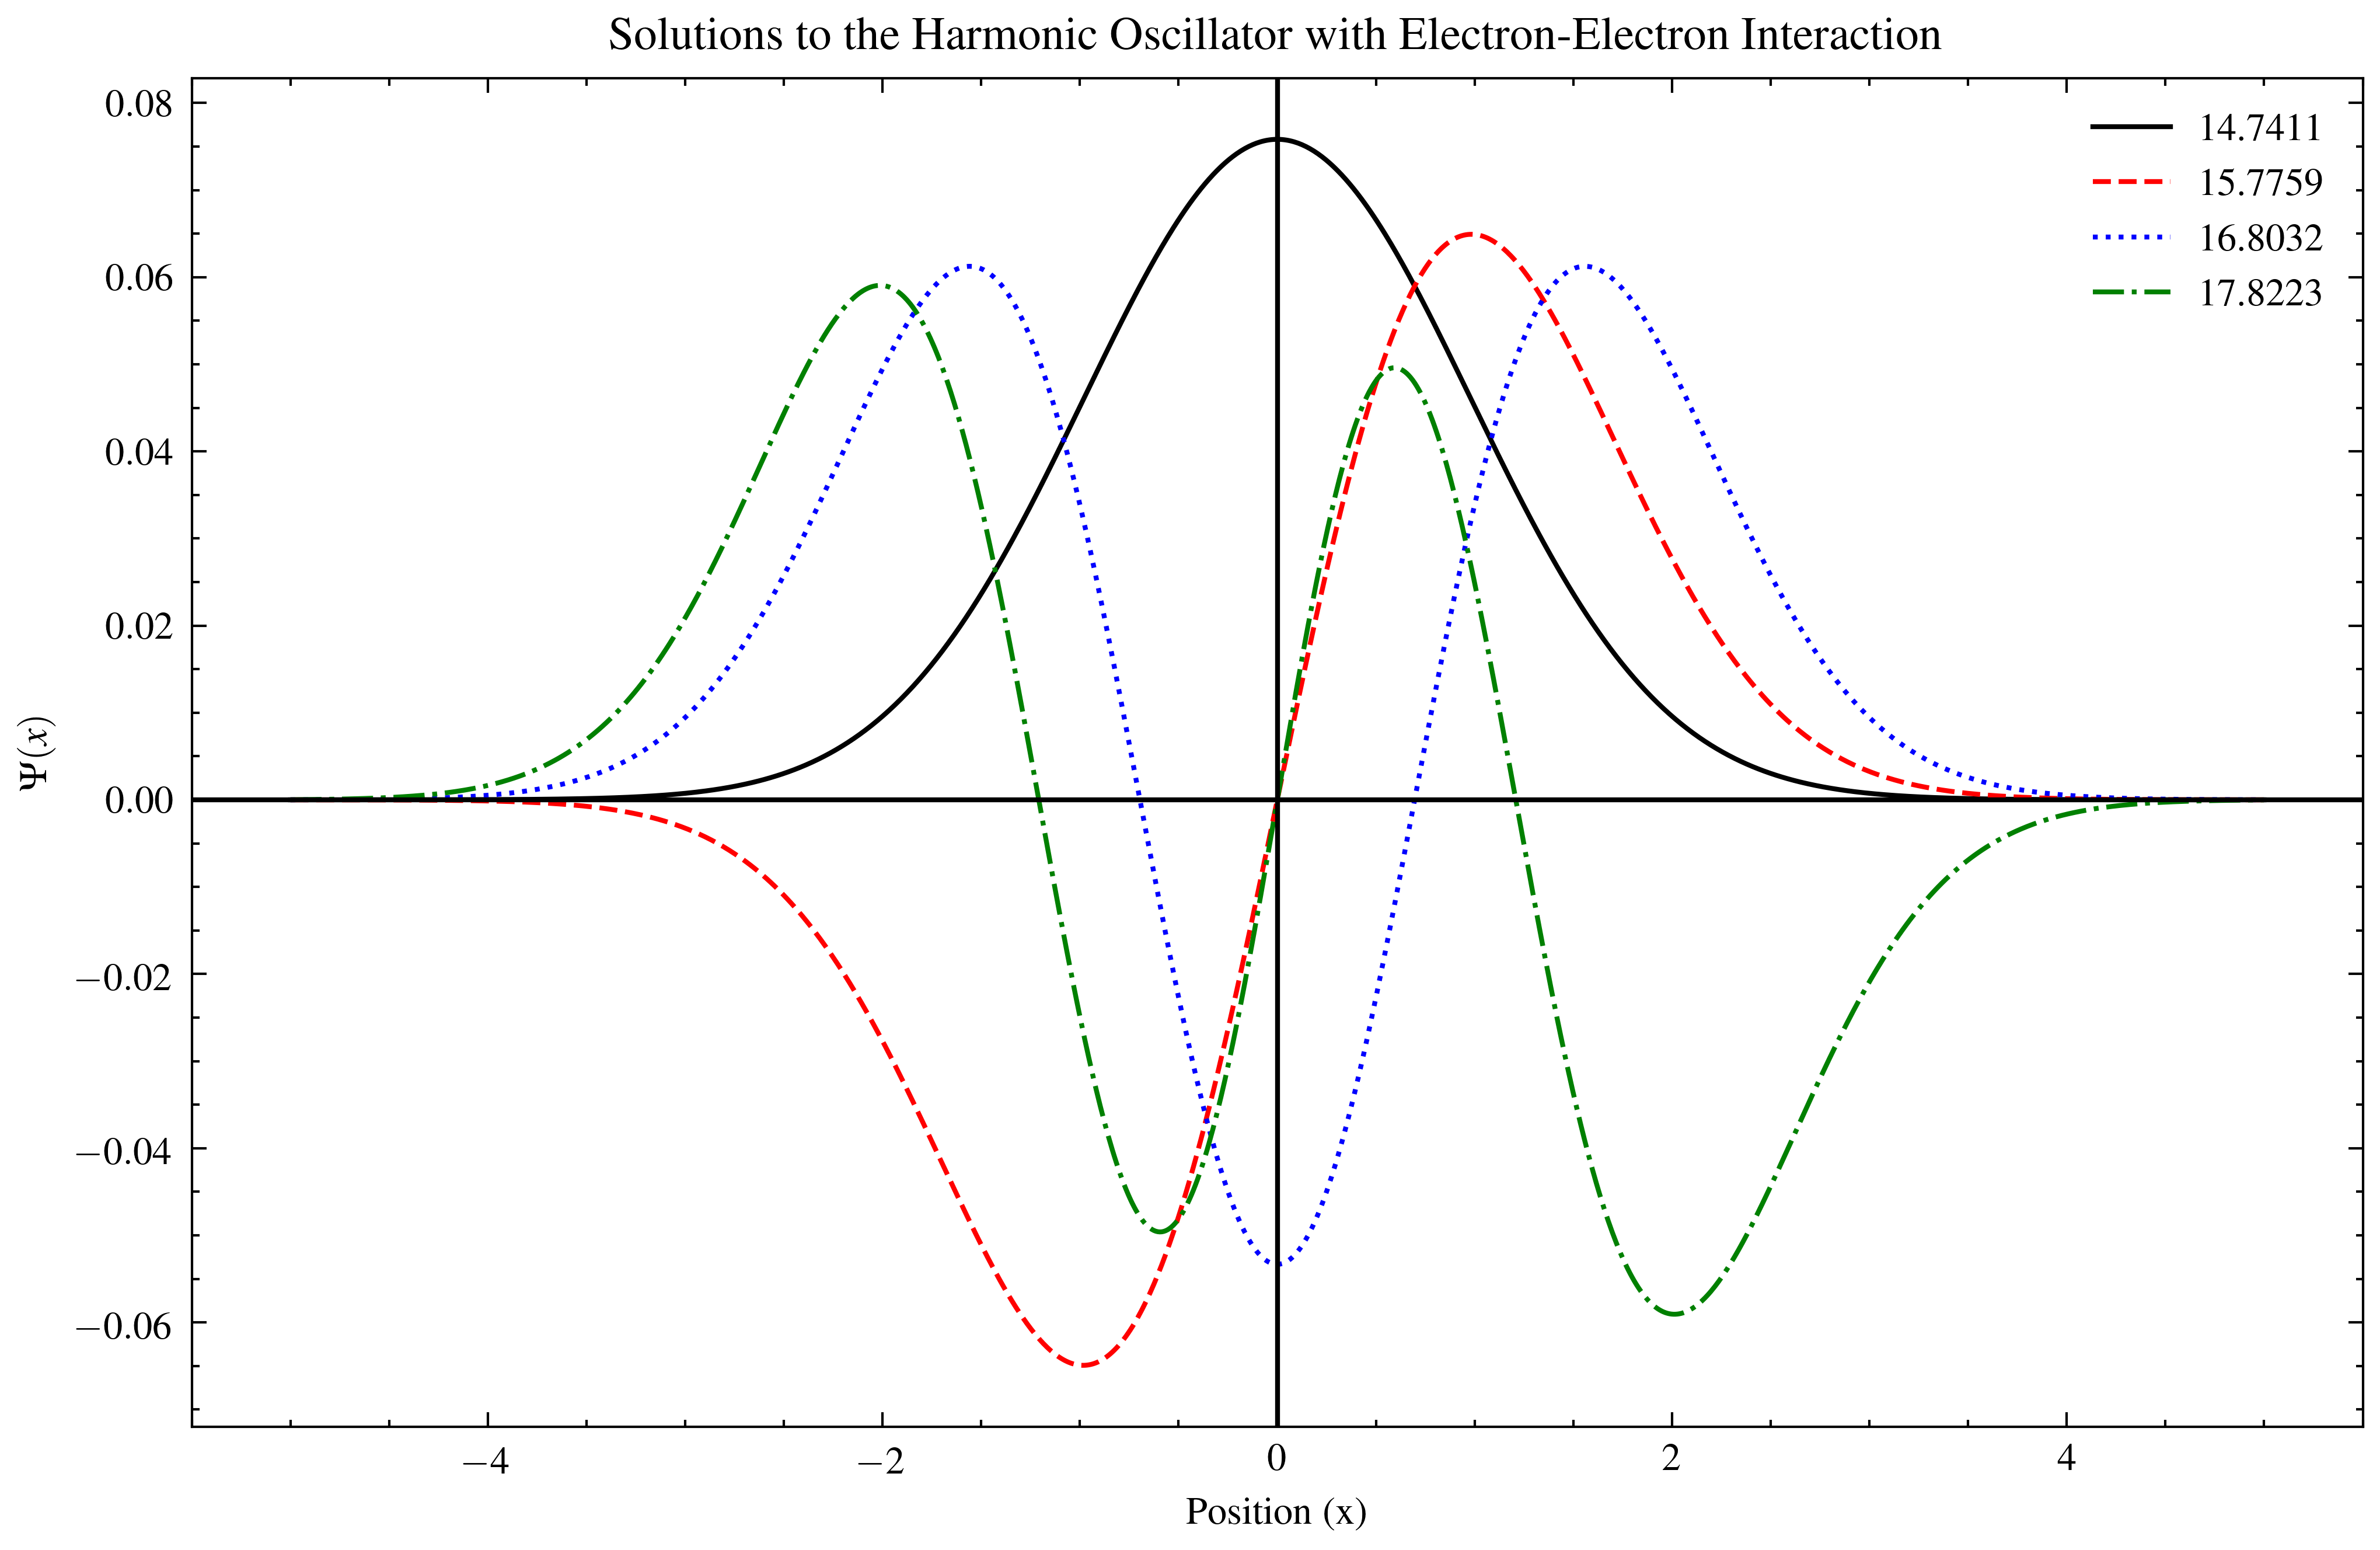
\includegraphics[width = \columnwidth]{Images/1DDFT.png}
    \caption{Solutions to the 1D DFT problem with LDA potential and Exchange Energy}
    \label{1d_dft}
\end{figure}


%%%%%%%%%%%%%%%%%%%%%%%%%%%%%%%%%%%%%%%%%%%%%%%%%%%%%%%%%%%%%%%%%%%%%%%%%%%%%
%%%%%%%%%%%%%%%%%%%%%%%%%%%%%%%%%%%%%%%%%%%%%%%%%%%%%%%%%%%%%%%%%%%%%%%%%%%%%
\section{\label{Conclusion}Conclusion and Discussions}

hihi-\cite{ROOT}
%%%%%%%%%%%%%%%%%%%%%%%%%%%%%%%%%%%%%%%%%%%%%%%%%%%%%%%%%%%%%%%%%%%%%%%%%%%%%
%%%%%%%%%%%%%%%%%%%%%%%%%%%%%%%%%%%%%%%%%%%%%%%%%%%%%%%%%%%%%%%%%%%%%%%%%%%%%

\end{multicols}
\bibliographystyle{plain}
\bibliography{bib.bib}


\end{document}